\chapter{On tree graphs and graph forests}
\label{sec:22}

\abstract*{ The chapter specifically addresses working with tree graphs and graph forests. We illustrate how to generate and recognize random tree graphs and how to compute the centres of a tree and draw a rooted and oriented tree. Finally, algorithms for computing spanning trees and forests are presented.}

\abstract{ The chapter specifically addresses working with tree graphs and graph forests. We illustrate how to generate and recognize random tree graphs and how to compute the centres of a tree and draw a rooted and oriented tree. Finally, algorithms for computing spanning trees and forests are presented. }

\section{Generating random tree graphs}
\label{sec:22.1}

Using the \texttt{RandomTree} class\index{RandomTree@\texttt{RandomTree} class} from the \texttt{graphs} module, we may, for instance, generate a random tree graph with 9 vertices.
\begin{lstlisting}[caption={Generating a random tree graph},label=list:22.1]
>>> from graphs import RandomTree
>>> rt = RandomTree(order=9,seed=100)
>>> rt
  *------- Graph instance description ----*
   Instance class   : RandomTree
   Instance name    : randomTree
   Graph Order      : 9
   Graph Size       : 8
   Valuation domain : [-1.00; 1.00]
   Attributes   : ['name', 'order',
                   'vertices', 'valuationDomain',
                   'edges', 'prueferCode',
                   'size', 'gamma']
   *---- RandomTree specific data ----*
   Pruefer code  : ['v3','v8','v8','v3','v7','v6','v7']
>>> rt.exportGraphViz('tutRandomTree')
  *---- exporting a dot file for GraphViz tools --*
   Exporting to tutRandomTree.dot
   neato -Tpng tutRandomTree.dot -o tutRandomTree.png
\end{lstlisting}
\begin{figure}[ht]
\sidecaption[t]
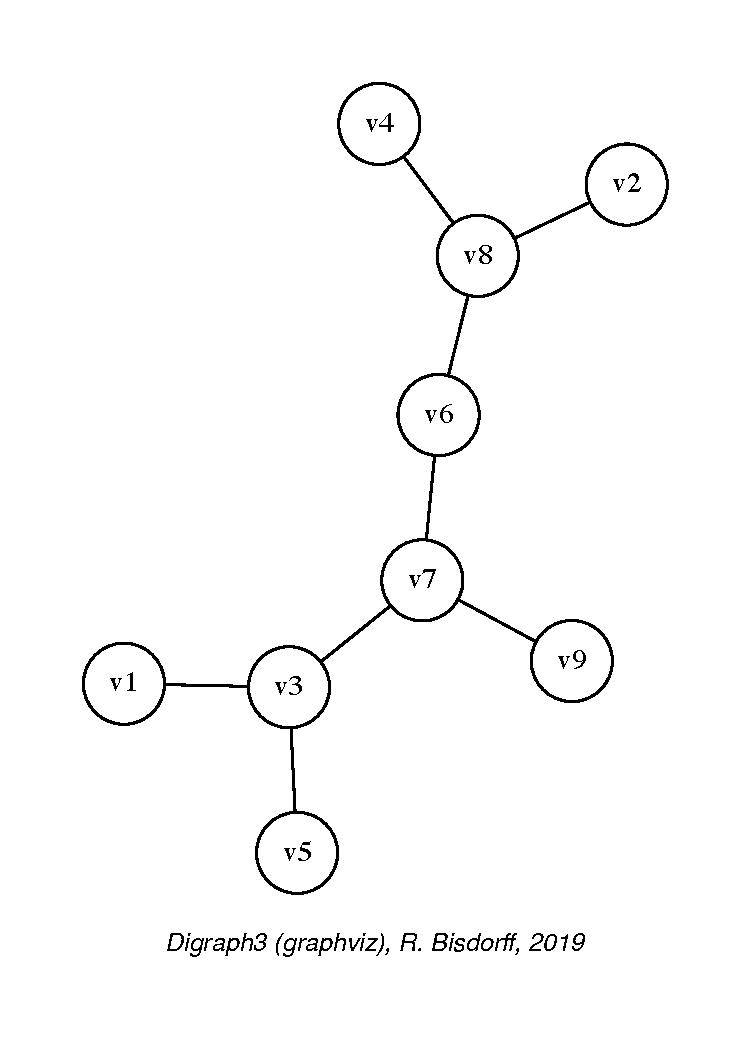
\includegraphics[width=6cm]{Figures/22-1-tutRandomTree.pdf}
\caption{Random tree graph instance of order 9. One may distinguish vertices like \texttt{v1}, \texttt{v2}, \texttt{v4}, \texttt{v5} or \texttt{v9}  of degree 1, called the \emph{leaves} of the tree, and vertices like \texttt{v3}, \texttt{v6}, \texttt{v7} or \texttt{v8} of degree 2 or more, called the \emph{nodes} of the tree} 
\label{fig:22.1}       % Give a unique label
\end{figure}

In Fig.~\vref{fig:22.1} one may notice that a tree graph of order $n > 2$ always contains $n-1$ edges (see Lines 7 and 8 in List.~\vref{list:22.1}) and its structure is entirely characterised by a corresponding \Pruefer \emph{code}, i.e. a list of vertices keys of length $n-2$. See, for instance in Line 15 the code \texttt{['v3'}, \texttt{'v8',} \texttt{'v8',} \texttt{'v3',} \texttt{'v7',} \texttt{'v6',} \texttt{'v7']} corresponding to our sample tree graph \texttt{rt}.

Each position of the code indicates the parent of the remaining leaf with the smallest vertex label. Vertex \texttt{v3} is thus the parent of \texttt{v1} and we drop leaf \texttt{v1}, \texttt{v8} is now the parent of leaf \texttt{v2} and we drop \texttt{v2}, vertex \texttt{v8} is again the parent of leaf \texttt{v4} and we drop \texttt{v4}, vertex \texttt{v3} is the parent of leaf \texttt{v5} and we drop \texttt{v5}, \texttt{v7} is now the parent of leaf \texttt{v3} and we may drop \texttt{v3}, \texttt{v6} becomes the parent of leaf \texttt{v8} and we drop \texttt{v8}, \texttt{v7} becomes the parent of leaf \texttt{v6} and we may drop \texttt{v6}. The two eventually remaining vertices, \texttt{v7} and \texttt{v9}, give the last link in the reconstructed tree \citep{JPB-1991}.  

It is, as well possible to, first, generate a random \Pruefer code of length $n-2$ from a set of $n$ vertices  (see List.~\vref{list:22.2} Lines 1-9 ) and then, construct the corresponding tree of order $n$ by reversing the procedure illustrated above. The resulting tree graph is shown in Fig.~\vref{fig:22.2}.
\begin{lstlisting}[caption={Generating a tree graph with a random \Pruefer code.},label=list:22.2]
>>> verticesList = ['v1','v2','v3','v4','v5','v6','v7']
>>> n = len(verticesList)
>>> from random import seed, choice
>>> seed(101)
>>> code = []
>>> for k in range(n-2):
...     code.append( choice(verticesList) )
>>> print(code)
  ['v5', 'v7', 'v2', 'v5', 'v3']
>>> rt = RandomTree(prueferCode=code)
>>> rt
  *------- Graph instance description ------*
   Instance class   : RandomTree
   Instance name    : randomTree
   Graph Order      : 7
   Graph Size       : 6
   Valuation domain : [-1.00; 1.00]
   Attributes : ['name', 'order', 'vertices',
                 'valuationDomain', 'edges',
                 'prueferCode', 'size', 'gamma']
  *---- RandomTree specific data ----*
   Pruefer code  : ['v5', 'v7', 'v2', 'v5', 'v3']
>>> rt.exportGraphViz('tutPruefTree')
  *---- exporting a dot file for GraphViz tools ---------*
   Exporting to tutPruefTree.dot
   neato -Tpng tutPruefTree.dot -o tutPruefTree.png
\end{lstlisting}
\begin{figure}[ht]
\sidecaption[t]
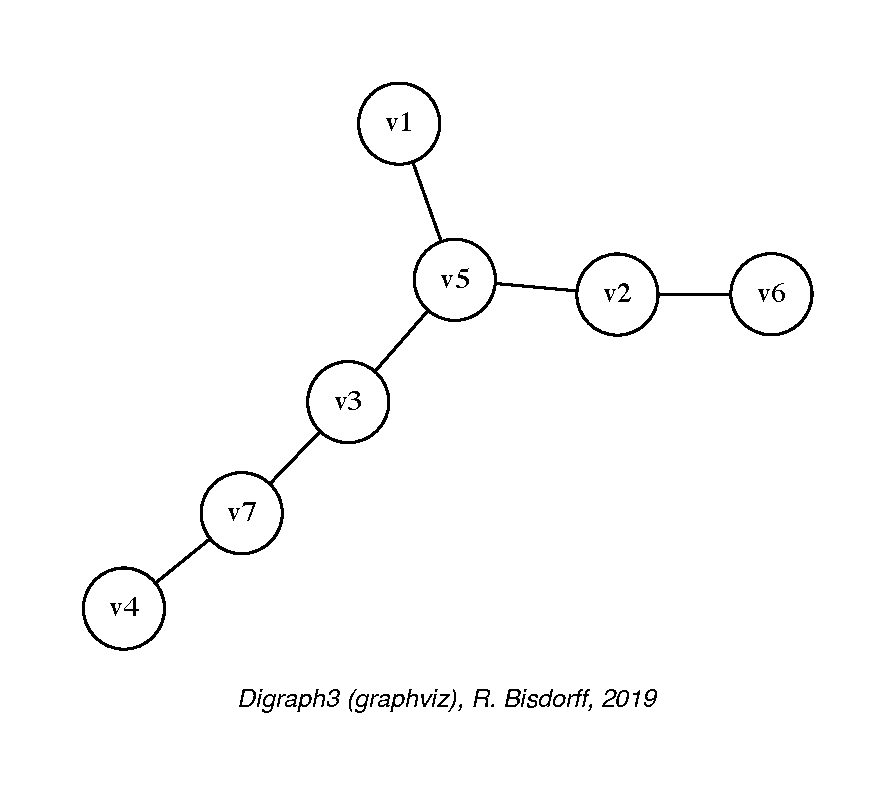
\includegraphics[width=7cm]{Figures/22-2-tutPruefTree.pdf}
\caption{Tree instance generated with a random \Pruefer code \texttt{['v5',} \texttt{'v7',} \texttt{'v2',} \texttt{'v5',} \texttt{'v3']}} 
\label{fig:22.2}       % Give a unique label
\end{figure}

Following from the bijection between a labelled tree and its \Pruefer code, we actually know that there exist $n^{n-2}$ different tree graphs with the same $n$ vertices.

Given a genuine graph, how can we recognize that it is in fact a tree instance ?

\section{Recognizing tree graphs}
\label{sec:22.2}

Given a graph \texttt{g} of order $n$ and size $s$, the following 5 assertions A1, A2, A3, A4 and A5 are all equivalent (see \citep{JPB-1991}):
\begin{itemize}
\item [A1] \texttt{g} is a tree;
\item [A2] \texttt{g} is without (chordless) cycles and $n \,=\, s + 1$;
\item [A3] \texttt{g} is connected and $n \,=\, s + 1$;
\item [A4] Any two vertices of \texttt{g} are always connected by a unique path;
\item [A5] \texttt{g} is connected and dropping any single edge will always disconnect \texttt{g}.
\end{itemize}

Assertion A3, for instance, gives a simple test for recognizing a tree graph. In case of a \emph{lazy evaluation} of the test in Listing~\vref{list:22.3} Line 3 below, it is opportune, from a computational complexity perspective, to first, check the order and size of the graph, before checking its potential connectedness. We provide the \texttt{isTree()} method\index{isTree@\texttt{isTree()}} for computing both these tests (see Line 8 in List.~\vref{list:22.3}).
\begin{lstlisting}[caption={Recognizing a tree graph.},label=list:22.3]
>>> from graphs import RandomGraph
>>> g = RandomGraph(order=8,edgeProbability=0.3,seed=62)
>>> if g.order == (g.size +1) and g.isConnected():
...     print('The graph is a tree ?', True)
... else:
...     print('The graph is a tree ?',False)   
  The graph is a tree ? True
>>> g.isTree()
  True  
\end{lstlisting}
The random graph of order $8$ and edge probability $30\%$, generated with seed $62$, is actually a tree graph instance, as confirmed by its graphviz drawing shown in Fig.~\vref{fig:22.3}.
\begin{lstlisting}
>>> g.exportGraphViz('test62')
  *---- exporting a dot file for GraphViz tools ---*
   Exporting to test62.dot
   fdp -Tpng test62.dot -o test62.png
\end{lstlisting}
\begin{figure}[ht]
\sidecaption[t]
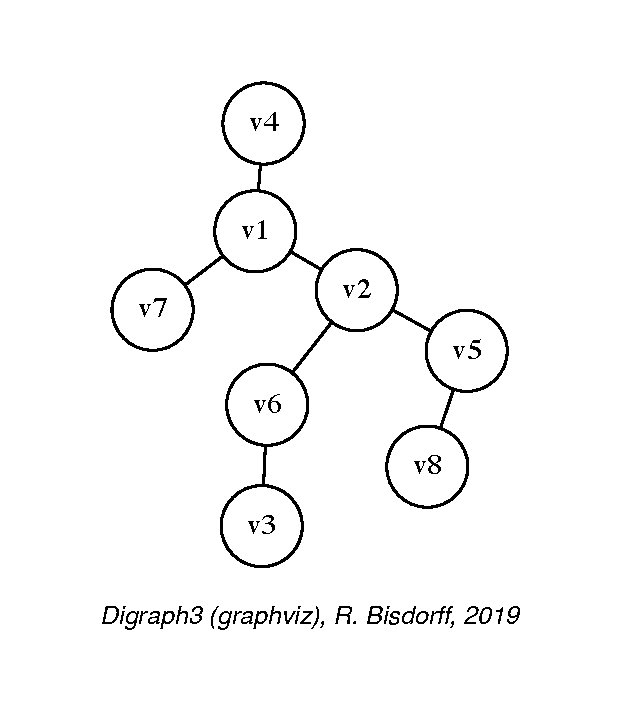
\includegraphics[width=7cm]{Figures/22-3-test62.pdf}
\caption{Recognizing a tree instance. We may notive that vertex \texttt{v2} is actually situated in the \emph{centre} of the tree with a neighborhood depth of 2} 
\label{fig:22.3}       % Give a unique label
\end{figure}

Yet, we still have to recover its corresponding \Pruefer code. Therefore, we may use the \texttt{tree2Pruefer()} method \index{tree2Pruefer@\texttt{tree2Pruefer()}} from the \texttt{TreeGraph} class. But, first, the instance class of graph \texttt{g} is changed to the \texttt{TreeGraph} type (see Line 2 in List.~\vref{list:22.4}). \index{TreeGraph@\texttt{TreeGraph()}}
\begin{lstlisting}[caption={Computing the \Pruefer code of a tree graph instance.},label=list:22.4]
>>> from graphs import TreeGraph
>>> g.__class__ = TreeGraph  
>>> g.tree2Pruefer()
  ['v6', 'v1', 'v2', 'v1', 'v2', 'v5']
\end{lstlisting}

In Fig.~\vref{fig:22.3}, we noticed that vertex \texttt{v2} is actually situated in the \emph{centre} of the tree with a neighborhood depth of 2. Centres of a graph are the vertices with minimal neighbourhood depth. For finding such centre(s), the \texttt{Graph} class provides the \texttt{computeGraphCentres()} method.\index{computeGraphCentres@\texttt{computeGraphCentres()}} (see Lines 1-2 in List.~\vref{list:22.4}). Knowing now the centre of graph \texttt{g}, we may draw a correspondingly rooted and oriented tree with the \texttt{exportOrientedTreeGraphViz()} method from the \texttt{TreeGraph} class (see Fig.~\vref{fig:22.4}.\index{exportOrientedTreeGraphViz@\texttt{exportOrientedTreeGraphViz()}}  
\begin{lstlisting}[caption={Computing the centres of a tree and drawing a rooted and oriented tree.},label=list:22.5]
>>> g.computeGraphCentres()
  {'v2': 2}
>>> g.exportOrientedTreeGraphViz(\
...       fileName='rootedTree', root='v2')
  *---- exporting a dot file for GraphViz tools
   Exporting to rootedTree.dot
   dot -Grankdir=TB -Tpng rootedTree.dot -o rootedTree.png
\end{lstlisting}
\begin{figure}[ht]
\sidecaption[t]
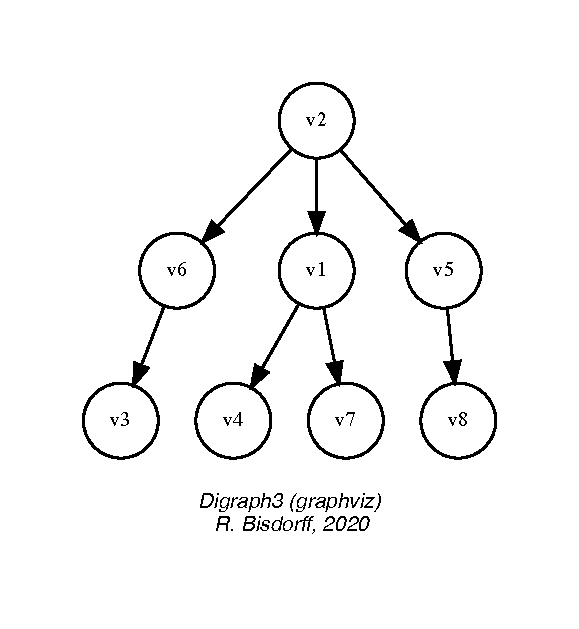
\includegraphics[width=6cm]{Figures/22-4-rootedTree.pdf}
\caption{Drawing an oriented tree rooted at its centre} 
\label{fig:22.4}       % Give a unique label
\end{figure}

Let us now turn our attention toward a major application of tree graphs, namely \emph{spanning trees} and \emph{forests} related to graph traversals.

\section{Spanning trees and forests}
\label{sec:22.2}

With the \texttt{RandomSpanningTree} class\index{RandomSpanningTree@\texttt{RandomSpanningTree} class} we may generate, from a given connected graph \texttt{g} instance, \emph{uniform} random instances of a spanning tree by using \Wilson's algorithm (see List.~\vref{list:22.6} and Fig.~\vref{fig:22.5}).
\begin{lstlisting}[caption={Generating uniform random spanning trees.},label=list:22.6]
>>> from graphs import RandomGraph,\
...                    RandomSpanningTree
>>> g = RandomGraph(order=9,\
...                 edgeProbability=0.4,seed=100)
>>> spt = RandomSpanningTree(g)
>>> spt
  *------- Graph instance description ------*
   Instance class   : RandomSpanningTree
   Instance name    : randomGraph_randomSpanningTree
   Graph Order      : 9
   Graph Size       : 8
   Valuation domain : [-1.00; 1.00]
   Attributes       : ['name','vertices','order',
                       'valuationDomain',
                       'edges','size','gamma',
                       'dfs','date', 'dfsx',
                       'prueferCode']
  *---- RandomTree specific data ----*
   Pruefer code  : ['v7','v9','v5','v1','v8','v4','v9']
>>> spt.exportGraphViz(fileName='randomSpanningTree',\
...                    WithSpanningTree=True)
  *---- exporting a dot file for GraphViz tools -----*
   Exporting to randomSpanningTree.dot
   [['v1','v5','v6','v5','v1','v8','v9','v3','v9','v4',
      'v7','v2','v7','v4','v9','v8','v1']]
   neato -Tpng randomSpanningTree.dot\
         -o randomSpanningTree.png
\end{lstlisting}
\begin{figure}[ht]
\sidecaption[t]
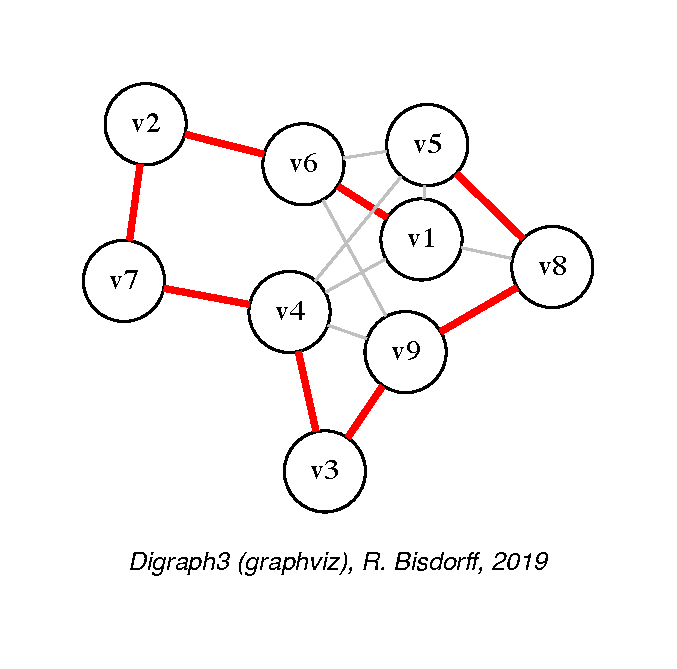
\includegraphics[width=7cm]{Figures/22-5-randomSpanningTree.pdf}
\caption{Random spanning tree} 
\label{fig:22.5}       % Give a unique label
\end{figure}

\Wilson's algorithm only works for connected graphs \citep{WIL-1996}. More general, and in case of a not connected graph, the \texttt{RandomSpanningForest} class\index{RandomSpanningForest@\texttt{RandomSpanningForest} class} generates a not necessarily uniform random instance of a \emph{spanning forest} --one or more random tree graphs-- generated from a random \emph{depth first search} of the graph components' traversals (see List.~\vref{list:22.7} and Fig.~\vref{fig:22.6}).
\begin{lstlisting}[caption={Computing spanning forests over disconnected graphs. },label=list:22.7]
>>> g = RandomGraph(order=15,\
...                 edgeProbability=0.1,seed=140)
>>> g.computeComponents()
  [{'v12','v01','v13'}, {'v02','v06'},
   {'v08','v03','v07'}, {'v15','v11','v10','v04','v05'},
   {'v09','v14'}]
>>> spf = RandomSpanningForest(g,seed=100)
>>> spf.exportGraphViz(fileName='spanningForest',\
...                    WithSpanningTree=True)
  *---- exporting a dot file for GraphViz tools -----*
    Exporting to spanningForest.dot
    [['v03','v07','v08','v07','v03'],
     ['v13','v12','v13','v01','v13'],
     ['v02','v06','v02'],
     ['v15','v11','v04','v11','v15',
            'v10','v05','v10','v15'],
     ['v09','v14','v09']]
  neato -Tpng spanningForest.dot -o spanningForest.png
\end{lstlisting}
\begin{figure}[ht]
\sidecaption[t]
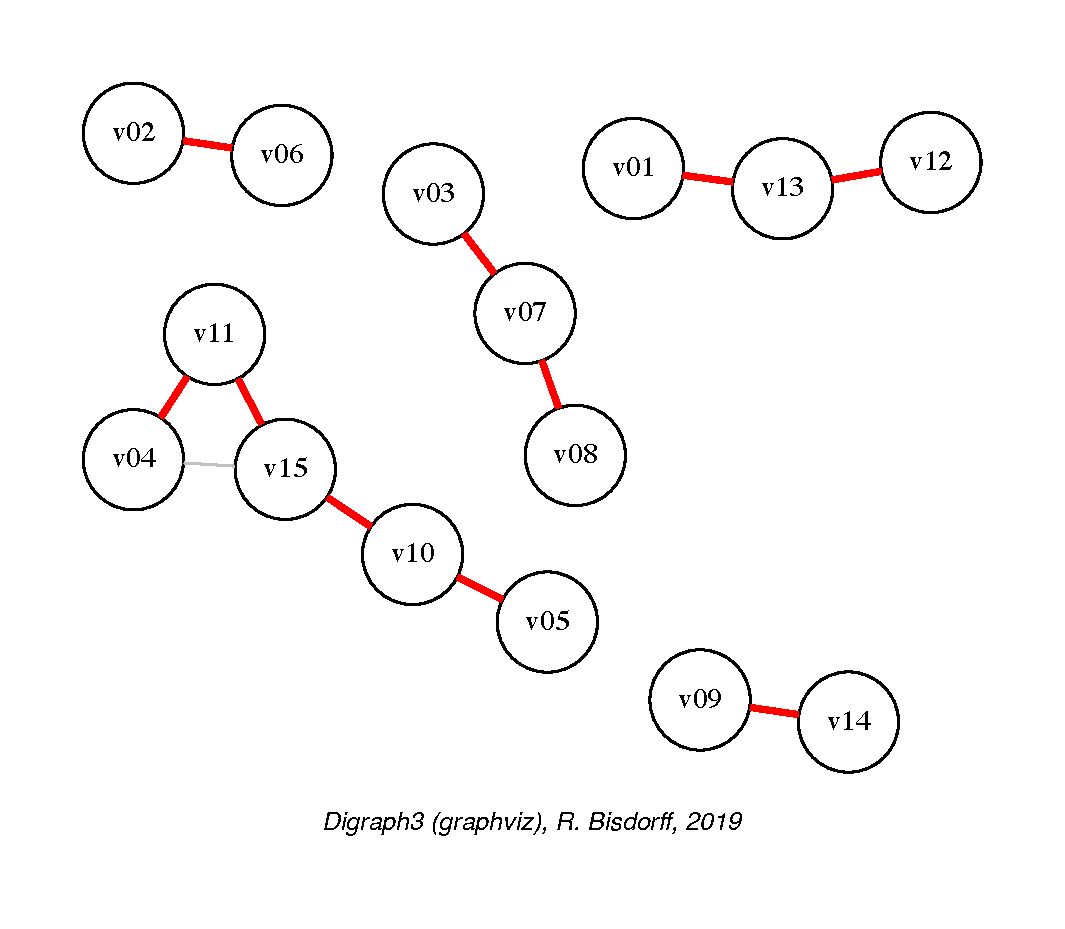
\includegraphics[width=7cm]{Figures/22-6-spanningForest.pdf}
\caption{Random spanning forest} 
\label{fig:22.6}       % Give a unique label
\end{figure}

\section{Maximum determined spanning forests}
\label{sec:22.3}

In case of valued graphs --supporting weighted edges-- we may finally construct a \emph{most determined} spanning tree (or forest if not connected) using \Kruskal's greedy minimum-spanning-tree algorithm on the dual valuation of the graph \citep{KRU-1956}\footnote{\Kruskal's algorithm is a minimum-spanning-tree algorithm which finds an edge of the least possible weight that connects any two trees in the forest.}.

In Listing~\vref{list:22.8} we generate, for instance, a randomly valued graph with five vertices and seven edges bipolar-valued in [-1.0; 1.0].\index{RandomValuationGraph@\texttt{RandomValuationGraph} class}
\begin{lstlisting}[caption={Generating randomly bipolar-valued graphs.},label=list:22.8]
>>> from graphs import RandomValuationGraph
>>> g = RandomValuationGraph(order=5,seed=2)
>>> g
  *------- Graph instance description ------*
   Instance class   : RandomValuationGraph
   Instance name    : randomGraph
   Graph Order      : 5
   Graph Size       : 7
   Valuation domain : [-1.00; 1.00]
   Attributes       : ['name', 'order',
                 'vertices', 'valuationDomain',
                 'edges', 'size', 'gamma']
\end{lstlisting}
To inspect the edges' actual weights, we first transform the graph into a corresponding digraph (see Line 1 in List.~\vref{list:22.9}) and use the \texttt{showRelationTable()} method (see Line 2) for printing its symmetric adjacency matrix. 
\begin{lstlisting}[caption={Symmetric relation table},label=list:22.9]
>>> dg = g.graph2Digraph()
>>> dg.showRelationTable()
  *---- Relation Table -----
    S   |  'v1'	 'v2'  'v3'  'v4'  'v5'	  
   -----|------------------------------
   'v1' |  0.00	 0.91  0.90 -0.89 -0.83	 
   'v2' |  0.91	 0.00  0.67  0.47  0.34	 
   'v3' |  0.90	 0.67  0.00 -0.38  0.21	 
   'v4' | -0.89	 0.47 -0.38  0.00  0.21	 
   'v5' | -0.83	 0.34  0.21  0.21  0.00	 
   Valuation domain: [-1.00;1.00]
\end{lstlisting}

To compute the most determined spanning tree or forest, we can use the \texttt{Best\-DeterminedSpanningForest} constructor.\index{BestDeterminedSpanningForest@\texttt{BestDeterminedSpanningForest} class}
\begin{lstlisting}[caption={Computing best determined spanning forests.},label=list:22.10]
>>> from graphs import\
                BestDeterminedSpanningForest
>>> mt = BestDeterminedSpanningForest(g)
>>> print(mt)
  *------- Graph instance description ------*
   Instance class   : BestDeterminedSpanningForest
   Instance name    : bdSpanningForest
   Graph Order      : 5
   Graph Size       : 4
   Valuation domain : [-1.00; 1.00]
   Attributes       : ['name','vertices','order',
                       'valuationDomain',
                       'edges','size','gamma',
                       'dfs','date',
                       'averageTreeDetermination']
  *---- best determined spanning tree  ----*
   Depth first search path(s) :
   [['v1','v2','v4','v2','v5','v2','v1','v3','v1']]
   Average determination(s) : [Decimal('0.655')]
\end{lstlisting}

The random graph \texttt{g} is connected and, hence, admits a single spanning tree of maximum mean determination = $(0.47 + 0.91 + 0.90 + 0.34)/4 = 0.655$ (see Lines 9, 6 and 10 in List.~\vref{list:22.8} and Fig.~\vref{fig:22.7}).
\begin{lstlisting}
>>> mt.exportGraphViz(\
...      fileName='bestDeterminedspanningTree',\
...      WithSpanningTree=True)
  *---- exporting a dot file for GraphViz tools ---*
   Exporting to spanningTree.dot
   [['v4','v2','v1','v3','v1','v2','v5','v2','v4']]
   neato -Tpng bestDeterminedSpanningTree.dot\
         -o bestDeterminedSpanningTree.png
\end{lstlisting}
\begin{figure}[ht]
\sidecaption[t]
\includegraphics[width=7cm]{Figures/22-7-bestDeterminedSpanningTree.pdf}
\caption{Best determined spanning tree} 
\label{fig:22.7}       % Give a unique label
\end{figure}

One may easily verify that all other potential spanning trees, including instead the edges \{\texttt{v3}, \texttt{v5}\} and/or \{\texttt{v4}, \texttt{v5}\}, will show a lower average determination.

\vspace{1cm}

Chapter~\ref{sec:23}, the last on undirected graphs, is devoted to different models of perfect graphs, namely split, interval, comparability and permutation graphs. 
 
%%%%%%% The chapter bibliography
%\normallatexbib
\clearpage
%\phantomsection
%\addcontentsline{toc}{section}{Chapter Bibliography}
\bibliographystyle{spbasic}
%\typeout{}
\bibliography{03-backMatters/reference}
%\chapter{On tree graphs and graph forests}
\label{sec:23}

\abstract*{}

\abstract{}

\section{Generating random tree graphs}
\label{aec:23.1}

Using the \texttt{RandomTree} class from the \texttt{graphs} module, we may, for instance, generate a random tree graph with 9 vertices.
\begin{lstlisting}
>>> from graphs import RandomTree
>>> t = RandomTree(order=9,seed=100)
>>> t
  *------- Graph instance description ----*
   Instance class   : RandomTree
   Instance name    : randomTree
   Graph Order      : 9
   Graph Size       : 8
   Valuation domain : [-1.00; 1.00]
   Attributes   : ['name', 'order',
                   'vertices', 'valuationDomain',
                   'edges', 'prueferCode',
                   'size', 'gamma']
   *---- RandomTree specific data ----*
   Pruefer code  : ['v3','v8','v8','v3','v7','v6','v7']
>>> t.exportGraphViz('tutRandomTree')
  *---- exporting a dot file for GraphViz tools --*
   Exporting to tutRandomTree.dot
   neato -Tpng tutRandomTree.dot -o tutRandomTree.png
\end{lstlisting}
\begin{figure}[h]
\sidecaption
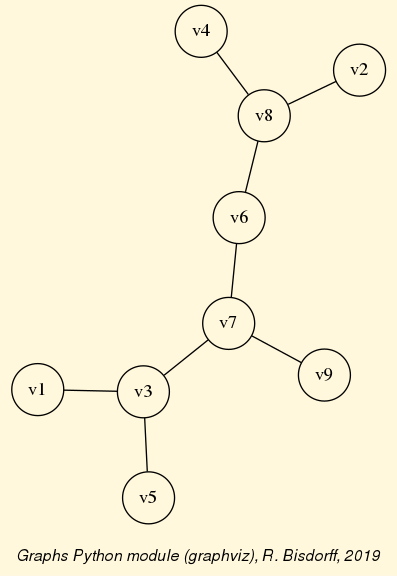
\includegraphics[width=6cm]{Figures/tutRandomTree.png}
\caption{Random tree graph instance of order 9} 
\label{fig:23.1}       % Give a unique label
\end{figure}

A tree graph of order $n$ contains $n-1$ edges (see Line 7 and 8) and we may distinguish vertices like 'v1', 'v2', 'v4', 'v5' or 'v9'  of degree 1, called the \emph{leaves} of the tree, and vertices like 'v3', 'v6', 'v7' or 'v8' of degree 2 or more, called the \emph{nodes} of the tree.

The structure of a tree graph of order $n > 2$ is entirely characterised by a corresponding \Pruefer \emph{code}, i.e. a list of vertices keys- of length $n-2$. See, for instance in Line 15 the code ['v3', 'v8', 'v8', 'v3', 'v7', 'v6', 'v7'] corresponding to our sample tree graph $t$.

Each position of the code indicates the parent of the remaining leaf with the smallest vertex label. Vertex 'v3' is thus the parent of 'v1' and we drop leaf 'v1', 'v8' is now the parent of leaf 'v2' and we drop 'v2', vertex 'v8' is again the parent of leaf 'v4' and we drop 'v4', vertex 'v3' is the parent of leaf 'v5' and we drop 'v5', 'v7' is now the parent of leaf 'v3' and we may drop 'v3', 'v6 becomes the parent of leaf 'v8' and we drop 'v8', 'v7' becomes now the parent of leaf 'v6' and we may drop 'v6'. The two eventually remaining vertices, 'v7' and 'v9', give the last link in the reconstructed tree (see [BAR-1991]).  

It is as well possible to first, generate a random \Pruefer code of length $n-2$ from a set of $n$ vertices and then, construct the corresponding tree of order $n$ by reversing the procedure illustrated above (see [BAR-1991]).
\begin{lstlisting}
>>> verticesList = ['v1','v2','v3','v4','v5','v6','v7']
>>> n = len(verticesList)
>>> from random import seed, choice
>>> seed(101)
>>> code = []
>>> for k in range(n-2):
...     code.append( choice(verticesList) )
>>> print(code)
  ['v5', 'v7', 'v2', 'v5', 'v3']
>>> t = RandomTree(prueferCode=['v5', 'v7', 'v2', 'v5', 'v3'])
>>> t
  *------- Graph instance description ------*
   Instance class   : RandomTree
   Instance name    : randomTree
   Graph Order      : 7
   Graph Size       : 6
   Valuation domain : [-1.00; 1.00]
   Attributes : ['name', 'order', 'vertices',
                 'valuationDomain', 'edges',
                 'prueferCode', 'size', 'gamma']
  *---- RandomTree specific data ----*
   Pruefer code  : ['v5', 'v7', 'v2', 'v5', 'v3']
>>> t.exportGraphViz('tutPruefTree')
  *---- exporting a dot file for GraphViz tools ---------*
   Exporting to tutPruefTree.dot
   neato -Tpng tutPruefTree.dot -o tutPruefTree.png
\end{lstlisting}
\begin{figure}[h]
\sidecaption
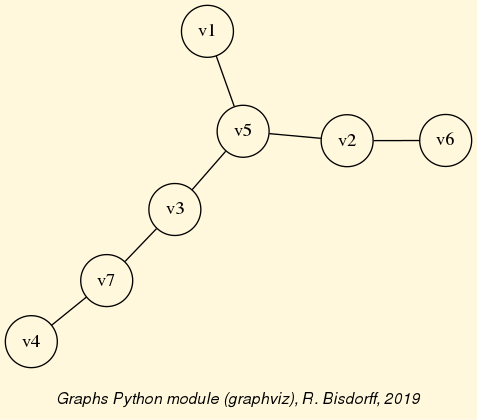
\includegraphics[width=7cm]{Figures/tutPruefTree.png}
\caption{Tree instance generated with a random \Pruefer code ['v5', 'v7', 'v2', 'v5', 'v3'].} 
\label{fig:23.2}       % Give a unique label
\end{figure}

Following from the bijection between a labelled tree and its \Pruefer code, we actually know that there exist $n^{n-2}$ different tree graphs with the same $n$ vertices.

Given a genuine graph, how can we recognize that it is in fact a tree instance ?

\section{Recognizing tree graphs}
\label{sec:23.2}

Given a graph $g$ of order $n$ and size $s$, the following 5 assertions A1, A2, A3, A4 and A5 are all equivalent (see [BAR-1991]):
\begin{itemize}
\item [A1] $g$ is a tree;
\item [A2] $g$ is without (chordless) cycles and $n \,=\, s + 1$;
\item [A3] $g$ is connected and $n \,=\, s + 1$;
\item [A4] Any two vertices of $g*$ are always connected by a unique path;
\item [A5] $g$ is connected and dropping any single edge will always disconnect $g$.
\end{itemize}
Assertion A3, for instance, gives a simple test for recognizing a tree graph. In case of a \emph{lazy evaluation} of the test in Line 3 below, it is opportune, from a computational complexity perspective, to first, check the order and size of the graph, before checking its potential connectedness.
\begin{lstlisting}
>>> from graphs import RandomGraph
>>> g = RandomGraph(order=8,edgeProbability=0.3,seed=62)
>>> if g.order == (g.size +1) and g.isConnected():
...     print('The graph is a tree ?', True)
... else:
...     print('The graph is a tree ?',False)   
  The graph is a tree ? True
\end{lstlisting}
The random graph of order 8 and edge probability $30\%$, generated with seed 62, is actually a tree graph instance, as we may readily confirm from its graphviz drawing in Fig. \ref{fig:23.3}.
\begin{lstlisting}
>>> g.exportGraphViz('test62')
  *---- exporting a dot file for GraphViz tools ---*
   Exporting to test62.dot
   fdp -Tpng test62.dot -o test62.png
\end{lstlisting}
\begin{figure}[h]
\sidecaption
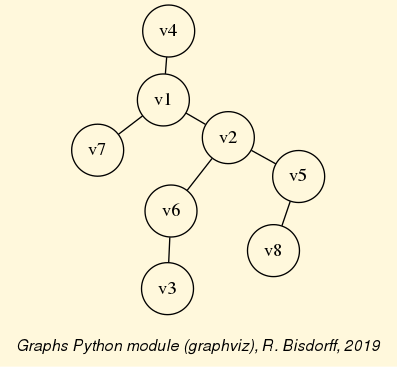
\includegraphics[width=7cm]{Figures/test62.png}
\caption{Recognizing a tree instance. We may notive that vertex 'v2' is actually situated in the \emph{centre} of the tree with a neighborhood depth of 2} 
\label{fig:23.3}       % Give a unique label
\end{figure}

Yet, we still have to recover its corresponding \Pruefer code. Therefore, we may use the \texttt{tree2Pruefer()} method.
\begin{lstlisting}
>>> from graphs import TreeGraph
>>> g.__class__ = TreeGraph
>>> g.tree2Pruefer()
  ['v6', 'v1', 'v2', 'v1', 'v2', 'v5']
\end{lstlisting}

In Fig. \ref{fig:23.3}, we also notice that vertex 'v2' is actually situated in the \emph{centre} of the tree with a neighborhood depth of 2. We may draw a correspondingly rooted and oriented tree graph.
\begin{lstlisting}
>>> g.computeGraphCentres()
     {'v2': 2}
>>> g.exportOrientedTreeGraphViz(\
...       fileName='rootedTree', root='v2')
  *---- exporting a dot file for GraphViz tools
   Exporting to rootedTree.dot
   dot -Grankdir=TB -Tpng rootedTree.dot -o rootedTree.png
\end{lstlisting}
\begin{figure}[h]
\sidecaption
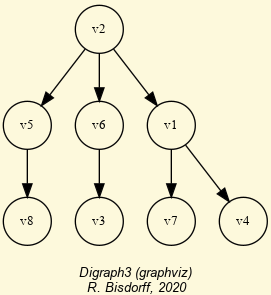
\includegraphics[width=6cm]{Figures/rootedTree.png}
\caption{Drawing an oriented tree rooted at its centre.} 
\label{fig:23.4}       % Give a unique label
\end{figure}

Let us now turn our attention toward a major application of tree graphs, namely \emph{spanning trees} and \emph{forests} related to graph traversals.

\section{Spanning trees and forests}
\label{sec:23.2}

With the \texttt{RandomSpanningTree} class we may generate, from a given connected graph $g$ instance, \emph{uniform} random instances of a spanning tree by using \Wilson's algorithm [WIL-1996] \footnote{\Wilson's algorithm only works for connected graphs.}
\begin{lstlisting}
>>> from graphs import RandomGraph,\
...                    RandomSpanningTree
>>> g = RandomGraph(order=9,\
...                 edgeProbability=0.4,seed=100)
>>> spt = RandomSpanningTree(g)
>>> spt
  *------- Graph instance description ------*
   Instance class   : RandomSpanningTree
   Instance name    : randomGraph_randomSpanningTree
   Graph Order      : 9
   Graph Size       : 8
   Valuation domain : [-1.00; 1.00]
   Attributes       : ['name','vertices','order',
                       'valuationDomain',
                       'edges','size','gamma',
                       'dfs','date', 'dfsx',
                       'prueferCode']
  *---- RandomTree specific data ----*
   Pruefer code  : ['v7','v9','v5','v1','v8','v4','v9']
>>> spt.exportGraphViz(fileName='randomSpanningTree',\
...                    WithSpanningTree=True)
  *---- exporting a dot file for GraphViz tools -----*
   Exporting to randomSpanningTree.dot
   [['v1','v5','v6','v5','v1','v8','v9','v3','v9','v4',
      'v7','v2','v7','v4','v9','v8','v1']]
   neato -Tpng randomSpanningTree.dot\
         -o randomSpanningTree.png
\end{lstlisting}
\begin{figure}[h]
\sidecaption
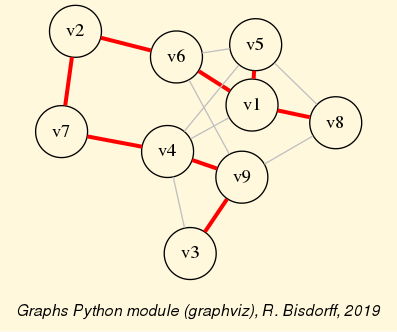
\includegraphics[width=7cm]{Figures/randomSpanningTree.png}
\caption{Random spanning tree} 
\label{fig:23.5}       % Give a unique label
\end{figure}

More general, and in case of a not connected graph, we may generate with the \emph{RandomSpanningForest} class a not necessarily uniform random instance of a \emph{spanning forest} --one or more random tree graphs-- generated from a random \emph{depth first search} of the graph components' traversals.
\begin{lstlisting}
>>> g = RandomGraph(order=15,\
...                 edgeProbability=0.1,seed=140)
>>> g.computeComponents()
  [{'v12','v01','v13'}, {'v02','v06'},
   {'v08','v03','v07'}, {'v15','v11','v10','v04','v05'},
   {'v09','v14'}]
>>> spf = RandomSpanningForest(g,seed=100)
>>> spf.exportGraphViz(fileName='spanningForest',\
...                    WithSpanningTree=True)
  *---- exporting a dot file for GraphViz tools -----*
    Exporting to spanningForest.dot
    [['v03','v07','v08','v07','v03'],
     ['v13','v12','v13','v01','v13'],
     ['v02','v06','v02'],
     ['v15','v11','v04','v11','v15',
            'v10','v05','v10','v15'],
     ['v09','v14','v09']]
  neato -Tpng spanningForest.dot -o spanningForest.png
\end{lstlisting}
\begin{figure}[h]
\sidecaption
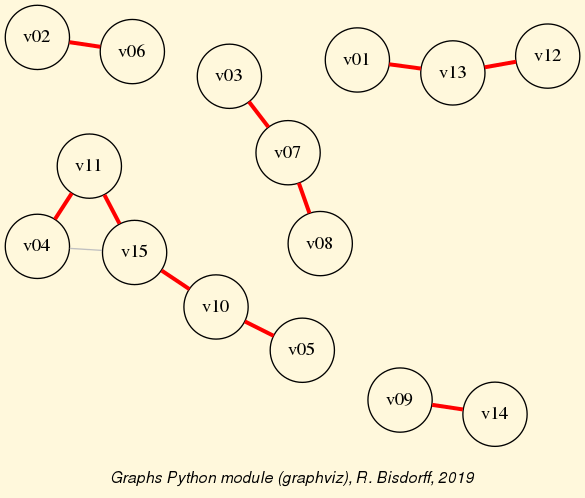
\includegraphics[width=8cm]{Figures/spanningForest.png}
\caption{Random spanning forest instance} 
\label{fig:23.6}       % Give a unique label
\end{figure}

\section{Maximum determined spanning forests}
\label{sec:23.3}

In case of valued graphs supporting weighted edges, we may finally construct a \emph{most determined} spanning tree (or forest if not connected) using \Kruskal's greedy minimum-spanning-tree algorithm Footnote[5] on the dual valuation of the graph [KRU-1956].

We consider, for instance, a randomly valued graph with five vertices and seven edges bipolar-valued in [-1.0; 1.0]. 
\begin{lstlisting}
>>> from graphs import RandomValuationGraph
>>> g = RandomValuationGraph(seed=2)
>>> g
  *------- Graph instance description ------*
   Instance class   : RandomValuationGraph
   Instance name    : randomGraph
   Graph Order      : 5
   Graph Size       : 7
   Valuation domain : [-1.00; 1.00]
   Attributes       : ['name', 'order',
                 'vertices', 'valuationDomain',
                 'edges', 'size', 'gamma']
\end{lstlisting}
To inspect the edges' actual weights, we first transform the graph into a corresponding digraph (see Line 1 below) and use the \texttt{showRelationTable()} method (see Line 2 below) for printing its symmetric adjacency matrix. 
\begin{lstlisting}[caption={Symmetric relation table},label=list:23.1]
>>> dg = g.graph2Digraph()
>>> dg.showRelationTable()
  *---- Relation Table -----
    S   |  'v1'	 'v2'  'v3'  'v4'  'v5'	  
   -----|------------------------------
   'v1' |  0.00	 0.91  0.90 -0.89 -0.83	 
   'v2' |  0.91	 0.00  0.67  0.47  0.34	 
   'v3' |  0.90	 0.67  0.00 -0.38  0.21	 
   'v4' | -0.89	 0.47 -0.38  0.00  0.21	 
   'v5' | -0.83	 0.34  0.21  0.21  0.00	 
   Valuation domain: [-1.00;1.00]
\end{lstlisting}

To compute the most determined spanning tree or forest, we may use the\texttt{BestDeterminedSpanningForest} constructor.
\begin{lstlisting}
>>> from graphs import\
                BestDeterminedSpanningForest
>>> mt = BestDeterminedSpanningForest(g)
>>> print(mt)
  *------- Graph instance description ------*
   Instance class   : BestDeterminedSpanningForest
   Instance name    : bdSpanningForest
   Graph Order      : 5
   Graph Size       : 4
   Valuation domain : [-1.00; 1.00]
   Attributes       : ['name','vertices','order',
                       'valuationDomain',
                       'edges','size','gamma',
                       'dfs','date',
                       'averageTreeDetermination']
  *---- best determined spanning tree  ----*
   Depth first search path(s) :
   [['v1','v2','v4','v2','v5','v2','v1','v3','v1']]
   Average determination(s) : [Decimal('0.655')]
\end{lstlisting}

The given graph is connected and, hence, admits a single spanning tree of maximum mean determination = $(0.47 + 0.91 + 0.90 + 0.34)/4 = 0.655$ (see Lines 9, 6 and 10 in Listing \ref{list:23.1} above).
\begin{lstlisting}
>>> mt.exportGraphViz(\
...      fileName='bestDeterminedspanningTree',\
...      WithSpanningTree=True)
  *---- exporting a dot file for GraphViz tools ---*
   Exporting to spanningTree.dot
   [['v4','v2','v1','v3','v1','v2','v5','v2','v4']]
   neato -Tpng bestDeterminedSpanningTree.dot\
         -o bestDeterminedSpanningTree.png
\end{lstlisting}
\begin{figure}[h]
\sidecaption
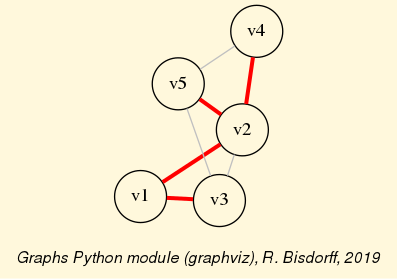
\includegraphics[width=7cm]{Figures/bestDeterminedSpanningTree.png}
\caption{Best determined spanning tree} 
\label{fig:23.7}       % Give a unique label
\end{figure}

One may easily verify that all other potential spanning trees, including instead the edges \{'v3','v5'\} and/or \{'v4','v5'\}, will show a lower average determination.
 
